\documentclass[aspectratio=169,usenames,dvipsnames]{beamer}

\usepackage{amsmath}
\usepackage{booktabs}
\usepackage{xcolor}
\usepackage[english]{babel}
\usepackage{unicode-math}
\usepackage{mathtools}
\usepackage{derivative}
\usepackage{makecell}
\usepackage{multirow}
\usepackage{siunitx}
\usepackage{pgfplots}
\usepackage{circuitikz}

\usetheme{metropolis}

\setmainfont{Stix Two Text}
\setmathfont{Stix Two Math}

\DeclarePairedDelimiter{\ceil}{\lceil}{\rceil}
\DeclarePairedDelimiter{\floor}{\lfloor}{\rfloor}
\DeclarePairedDelimiter{\abs}{\lvert}{\rvert}
\DeclarePairedDelimiter{\norm}{\lVert}{\rVert}
\DeclarePairedDelimiter{\bra}{\langle}{\rvert}
\DeclarePairedDelimiter{\ket}{\lvert}{\rangle}
\DeclarePairedDelimiter{\expval}{\langle}{\rangle}
\DeclarePairedDelimiter{\norder}{\mathcolon}{\mathcolon}
\DeclarePairedDelimiter{\anorder}{\typecolon}{\typecolon}
	
\newcommand{\laplace}{\mbfnabla^2}
\newcommand{\trans}{{\scriptscriptstyle\mathsf{T}}}

\newcommand{\conv}{\ast}
\newcommand{\vdot}{\cdot}
\newcommand{\vcross}{\vectimes}
\newcommand{\vb}[1]{\symbfup{#1}}
\newcommand{\vu}[1]{\hat{\vb{#1}}}
\newcommand*\dd[2][\relax]{\mathop{\ifx\relax#1\odif{#2}\else \odif[order={#1}]{#2}\fi}}

\newcommand{\vacket}{\ket*{0}}
\newcommand{\vacbra}{\bra*{0}}

\DeclareMathOperator{\trace}{Tr}
\DeclareMathOperator{\sinc}{sinc}

\AtBeginDocument{
	\let\Re\relax
	\let\Im\relax
	\DeclareMathOperator{\Re}{Re}
	\DeclareMathOperator{\Im}{Im}

	\renewcommand{\div}{\mathop{\mbfnabla\vdot}}
	\newcommand{\curl}{\mathop{\mbfnabla\vectimes}}
}

\DeclarePairedDelimiterX{\comm}[2]{[}{]}{#1,#2}

\DeclarePairedDelimiterX{\braket}[2]{\langle}{\rangle}{#1\delimsize\vert#2}
\DeclarePairedDelimiterX{\ketbra}[1]{\lvert}{\rvert}{#1\rangle\delimsize\langle#1}


\pgfplotsset{compat=1.17}
\usetikzlibrary{arrows.meta}
\usetikzlibrary{fit}
\usetikzlibrary{positioning}
\usetikzlibrary{shapes.geometric}
\usetikzlibrary{shapes.misc}
\usepgfplotslibrary{groupplots}

\definecolor{exotic orange}{RGB}{255,128,0}
\definecolor{exotic green}{RGB}{0,102,102}
\definecolor{exotic blue}{RGB}{67,132,161}
\definecolor{exotic red}{RGB}{250,86,86}

\DeclareSIUnit{\arbitraryunit}{arb. unit}

\title{A theoretical framework for CV-QKD}
\date{\today}
\author{Bodo Kaiser}
\institute{Ludwig-Maximilians-Universität München}

\begin{document}

	\maketitle

	\begin{frame}
		\begin{quote}
			You never know what you might discover by thinking outside the box that culture, conformity, and critics have tried to impose. --- T.D. Jakes
		\end{quote}
	\end{frame}
	
	% why is QKD interesting? -> intersection of multiple disciplines (quantum information theory, quantum optics, communication engineering)	
	\begin{frame}{Outline}
		\begin{columns}[c, onlytextwidth]
			\column{0.6\textwidth}
			\begin{figure}
				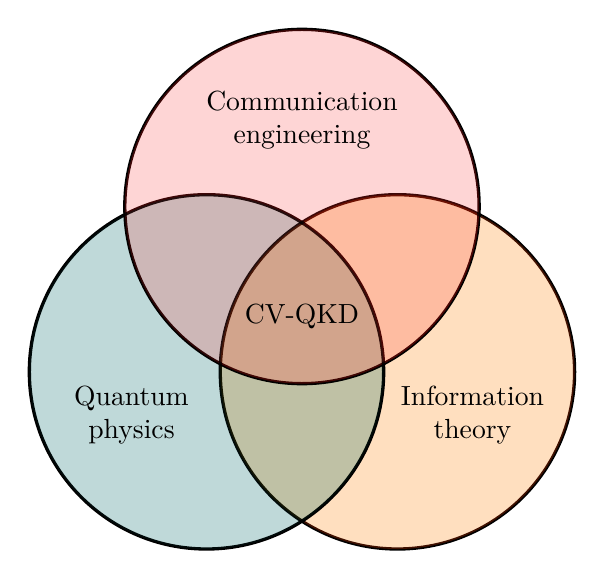
\begin{tikzpicture}[
					venn circle/.style={draw, very thick, fill opacity=0.25, circle, minimum width=45mm},
					venn label/.style={align=center},
				]
					\begin{scope}[blend group=soft light]
						\node[venn circle, fill=exotic red] (qp) at (90:1.4) {};
						\node[venn circle, fill=exotic green] (it) at (210:1.4) {};
						\node[venn circle, fill=exotic orange] (qp) at (330:1.4) {};
					\end{scope}
					
					\node[venn label] {CV-QKD};
					\node[venn label] at (90:2.5) {Communication\\engineering};
					\node[venn label] at (210:2.5) {Quantum\\physics};
					\node[venn label] at (330:2.5) {Information\\theory};
				\end{tikzpicture}
			\end{figure}

			\column{0.4\textwidth}
			\setbeamertemplate{section in toc}[sections numbered]
			\tableofcontents[hideallsubsections]
		\end{columns}
	\end{frame}
	
	\section{Introduction}

	% what is secure communication: integrity and confidentiality	
	% key distribution problem
	% public-key distribution
	% information-theoretical secure for OTP but practically one uses AES
	\begin{frame}{Secure transmission system}
		\begin{figure}
			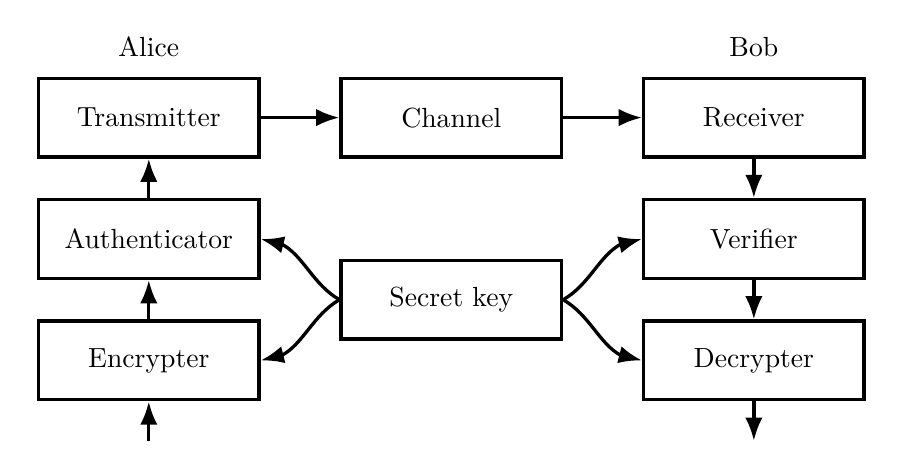
\begin{tikzpicture}[
				node distance=5mm,
				arrow/.style={very thick, -Latex},
				block/.style={draw, very thick, minimum width=28mm, minimum height=10mm},		
			]
				\coordinate (in);
				\node[block, above=of in] (encryption) {Encrypter};
				\node[block, above=of encryption] (authentication) {Authenticator};
				\node[block, above=of authentication] (transmitter) {Transmitter};
				\node[block, right=10mm of transmitter] (channel) {Channel};
				\node[block, right=10mm of channel] (receiver) {Receiver};
				\node[block, below=of receiver] (verification) {Verifier};
				\node[block, below=of verification] (decryption) {Decrypter};
				\coordinate[below=of decryption] (out);
	
				\path (encryption) -- (verification) node[midway, block, align=center] (key) {Secret key};
	
				\draw[arrow] (key.west) to[out=210, in=0] (encryption.east);
				\draw[arrow] (key.west) to[out=150, in=0]  (authentication.east);
				\draw[arrow] (key.east) to[out=-30, in=180] (decryption.west);
				\draw[arrow] (key.east) to[out=30, in=180] (verification.west);

				\draw[arrow] (in) -- (encryption);
				\draw[arrow] (encryption) -- (authentication);
				\draw[arrow] (authentication) -- (transmitter);
				
				\draw[arrow] (decryption) -- (out);
				\draw[arrow] (verification) -- (decryption);
				\draw[arrow] (receiver) -- (verification);
		
				\draw[arrow] (transmitter) -- (channel.west);
				\draw[arrow] (channel.east) -- (receiver);
				
				\node[label={Alice}, fit=(encryption) (transmitter)] {};
				\node[label={Bob}, fit=(decryption) (receiver)] {};
			\end{tikzpicture}
			\caption{Block diagram of a secure transmission system.}
		\end{figure}
	\end{frame}

    % quantum transmission (random seed, correlated data)
	% post-processing (shared secret key from correlated data)
	\begin{frame}{Quantum key distribution system}
		\begin{figure}
			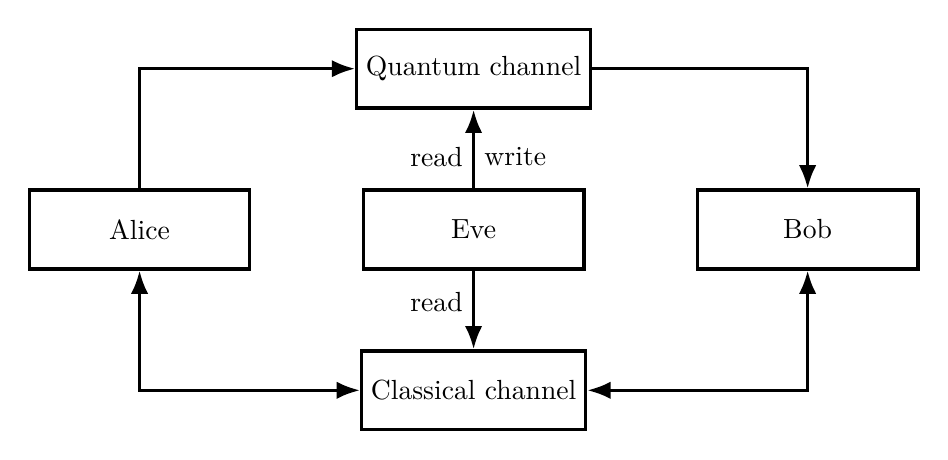
\begin{tikzpicture}[
				node distance=5mm,
				arrow/.style={very thick, -Latex},
				block/.style={draw, very thick, minimum width=28mm, minimum height=10mm},
			]
				\node[block] (alice) {Alice};
				\node[block, right=14mm of alice] (eve) {Eve};
				\node[block, above=10mm of eve] (quantum channel) {Quantum channel};
				\node[block, below=10mm of eve] (classical channel) {Classical channel};
				\node[block, right=14mm of eve] (bob) {Bob};

				\draw[arrow] (eve) -- (classical channel) node[midway, left, yshift=1mm] {read};
				\draw[arrow] (eve) -- (quantum channel) node[midway, left, yshift=-1mm] {read} node[midway, right, yshift=-1mm] {write};
				\draw[arrow] (alice.north) -- (alice.north|-quantum channel.west) -- (quantum channel.west);
				\draw[arrow, Latex-Latex] (alice.south) -- (alice.south|-classical channel.west) -- (classical channel.west);
				\draw[arrow] (quantum channel.east) -- (quantum channel.east-|bob.north) -- (bob.north);
				\draw[arrow, Latex-Latex] (classical channel.east) -- (classical channel.east-|bob.south) -- (bob.south);
			\end{tikzpicture}
			\caption{Block diagram of a quantum key distribution (QKD) system.}
		\end{figure}
	\end{frame}
	
	\begin{frame}{Discrete and continuous-variable QKD}
		\begin{table}[htb]
			\caption{Comparison of discrete- and continuous-variable QKD.}
			\begin{tabular}{lcc}
				\toprule
					& Discrete & Continuous \\
				\midrule
					Visualization & Bloch sphere & Phase space \\
					Hilbert space (dim) & Finite (two) & Countable (infinite) \\
					Observable & $\vb{\hat{S}}(\vb{n})=\hat{S}_in^i$ & $\hat{X}(\vartheta)=\frac{1}{\sqrt{2}}\left(\hat{a}e^{-i\vartheta}+\hat{a}^\dagger e^{+i\vartheta}\right)$ \\
					Standard basis & $\left\{\ket{0},\ket{1}\right\}$ & $\left\{\ket{x},\ket{p}\right\}_{x,p\in\mathbb{R}}$ \\
				\bottomrule
			\end{tabular}
		\end{table}
	\end{frame}
	
	\begin{frame}{Continuous-variable QKD using coherent states}
		\begin{figure}
			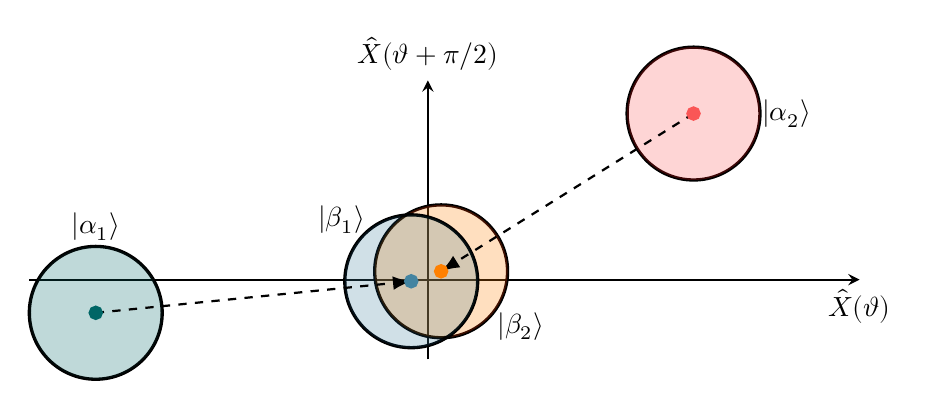
\begin{tikzpicture}[
				var/.style={draw, very thick, fill opacity=0.25, circle, minimum width=45mm},
			]
				\begin{axis}[
					height=6cm,
					width=\linewidth,
					clip=false,
					axis lines=center,
					axis equal image,
					axis line style=thick,
					xlabel={$\hat{X}(\vartheta)$},
					ylabel={$\hat{X}(\vartheta+\pi/2)$},
					ticks=none,
					xmin=-6,
					xmax=+6.5,
					ymin=-1.2,
					ymax=+3,
					axis line style={thick},
					x label style={anchor=north},
					y label style={anchor=south},
				]
					\begin{scope}[blend group=soft light]					
						\draw[var, fill=exotic green] (axis cs:-5,-0.5) circle (1);
						\draw[var, fill=exotic red] (axis cs:4,2.5) circle (1);
						
						\draw[var, fill=exotic blue] (axis cs:-0.25,-0.025) circle (1);
						\draw[var, fill=exotic orange] (axis cs:0.2,0.125) circle (1);
					\end{scope}

					\addplot[very thick, mark=*, exotic green] coordinates {(-5,-0.5)};
					\addplot[very thick, mark=*, exotic red] coordinates {(4,2.5)};					
					\addplot[very thick, mark=*, exotic blue] coordinates {(-0.25,-0.025)};
					\addplot[very thick, mark=*, exotic orange] coordinates {(0.2,0.125)};
					
					\node at (axis cs:-5,0.8) {$\ket{\alpha_1}$};
					\node at (axis cs:5.4,2.5) {$\ket{\alpha_2}$};
					\node at (axis cs:-1.3,0.9) {$\ket{\beta_1}$};
					\node at (axis cs:1.4,-0.7) {$\ket{\beta_2}$};
		
					\draw[-Latex, dashed, thick] (axis cs:-5,-0.5) -- (axis cs:-0.25,-0.025);
					\draw[-Latex, dashed, thick] (axis cs:4,2.5) -- (axis cs:0.2,0.125);
				\end{axis}
			\end{tikzpicture}
			\caption{Phase space diagram of transmitted and received coherent states with mean (dots) and variances (opaque circles).}
		\end{figure}
	\end{frame}
	
	\begin{frame}{Continuous-variable QKD using continuous-time coherent states}
		\begin{figure}
			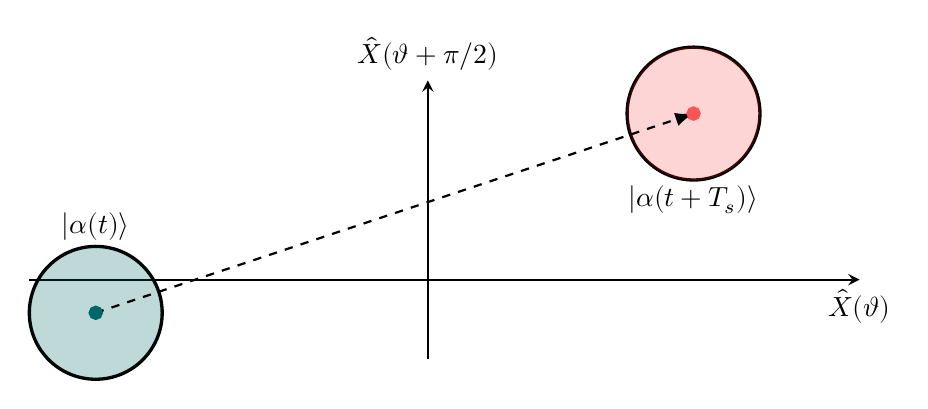
\begin{tikzpicture}[
				var/.style={draw, very thick, fill opacity=0.25, circle, minimum width=45mm},
			]
				\begin{axis}[
					height=6cm,
					width=\linewidth,
					clip=false,
					axis lines=center,
					axis equal image,
					axis line style=thick,
					xlabel={$\hat{X}(\vartheta)$},
					ylabel={$\hat{X}(\vartheta+\pi/2)$},
					ticks=none,
					xmin=-6,
					xmax=+6.5,
					ymin=-1.2,
					ymax=+3,
					axis line style={thick},
					x label style={anchor=north},
					y label style={anchor=south},
				]
					\begin{scope}[blend group=soft light]					
						\draw[var, fill=exotic green] (axis cs:-5,-0.5) circle (1);
						\draw[var, fill=exotic red] (axis cs:4,2.5) circle (1);
					\end{scope}

					\addplot[very thick, mark=*, exotic green] coordinates {(-5,-0.5)};
					\addplot[very thick, mark=*, exotic red] coordinates {(4,2.5)};
					
					\node at (axis cs:-5,0.8) {$\ket{\alpha(t)}$};
					\node at (axis cs:4,1.2) {$\ket{\alpha(t+T_s)}$};
					\draw[-Latex, dashed, thick] (axis cs:-5,-0.5) -- (axis cs:4,2.5);
				\end{axis}
			\end{tikzpicture}
			\caption{Phase space diagram of continuous-time coherent states with mean (dots) and variances (opaque circles) at two time instances.}
		\end{figure}
	\end{frame}

	\begin{frame}{Software-defined transmission system}
		\begin{figure}
			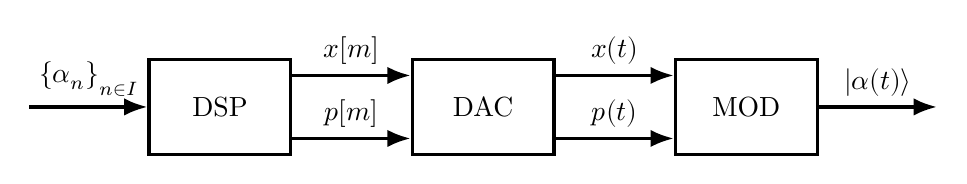
\begin{tikzpicture}[
				node distance=15mm,
				arrow/.style={very thick, -Latex},
				block/.style={draw, very thick, minimum width=18mm, minimum height=12mm},
			]
				\coordinate (in) at (0,0);
				\node (dsp) [block, right=of in] {DSP};
				\node (dac) [block, right=of dsp] {DAC};
				\node (mod) [block, right=of dac] {MOD};
				\coordinate[right=of mod] (out);
				
				\draw[arrow] (in) -- (dsp) node[midway, above] {$\left\{\alpha_n\right\}_{n\in I}$};
				\draw[arrow] ([yshift=4mm]dsp.east) -- ([yshift=4mm]dac.west) node[midway, above] {$x[m]$};
				\draw[arrow] ([yshift=-4mm]dsp.east) -- ([yshift=-4mm]dac.west) node[midway, above] {$p[m]$};
				\draw[arrow] ([yshift=4mm]dac.east) -- ([yshift=4mm]mod.west) node[midway, above] {$x(t)$};
				\draw[arrow] ([yshift=-4mm]dac.east) -- ([yshift=-4mm]mod.west) node[midway, above] {$p(t)$};
				\draw[arrow] (mod) -- (out) node[midway, above] {$\ket{\alpha(t)}$};
			\end{tikzpicture}
			\caption{Block diagram of the software-defined transmitter architecture.}
		\end{figure}
		
		\begin{figure}
			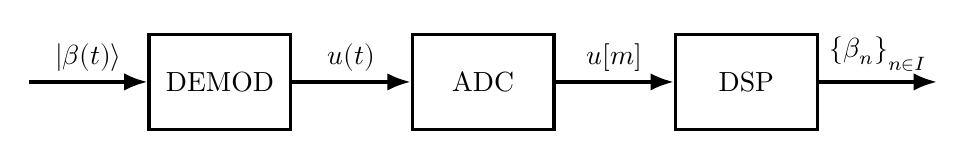
\begin{tikzpicture}[
				node distance=15mm,
				arrow/.style={very thick, -Latex},
				block/.style={draw, very thick, minimum width=18mm, minimum height=12mm},
			]
				\coordinate (in) at (0,0);
				\node (dsp) [block, right=of in] {DEMOD};
				\node (dac) [block, right=of dsp] {ADC};
				\node (mod) [block, right=of dac] {DSP};
				\coordinate[right=of mod] (out);
				
				\draw[arrow] (in) -- (dsp) node[midway, above] {$\ket{\beta(t)}$};
				\draw[arrow] (dsp.east) -- (dac.west) node[midway, above] {$u(t)$};
				\draw[arrow] (dac.east) -- (mod.west) node[midway, above]{$u[m]$};
				\draw[arrow] (mod) -- (out) node[midway, above] {$\left\{\beta_n\right\}_{n\in I}$};
			\end{tikzpicture}
			\caption{Block diagram of software-defined receiver architecture.}
		\end{figure}
	\end{frame}

	\section{Coherent state transmitter}
	
	\begin{frame}{Digital signal processing pipeline for symbol encoding}
		\begin{figure}
			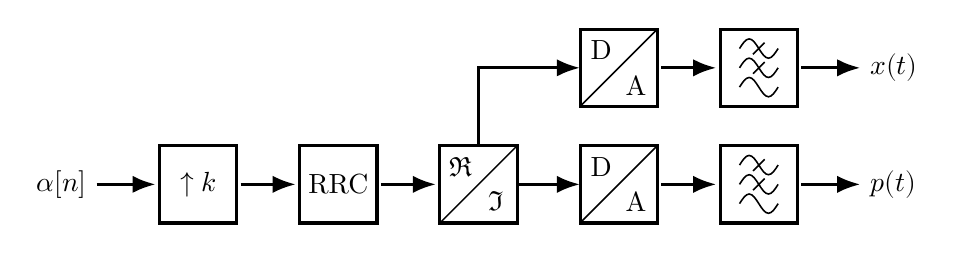
\begin{tikzpicture}[
				line width=0.2mm,
				node distance=8mm,
				arrow/.style={very thick, -Latex},
			]
				\node (in) {$\alpha[n]$};
				\node (up) [twoportshape, right=of in, t={$\uparrow k$}] {};
				\node (rrc) [twoportshape, right=of up, t=RRC] {};
				\node (real) [twoportsplitshape, circuitikz/t1={$\Re$}, circuitikz/t2={$\Im$}, right=of rrc] {};

				\node (dacp) [dacshape, right=of real] {};
				\node (lowp) [lowpassshape, right=of dacp] {};
				\node (outp) [right=of lowp] {$p(t)$};
				
				\node (dacx) [dacshape, above=5mm of dacp] {};
				\node (lowx) [lowpassshape, right=of dacx] {};
				\node (outx) [right=of lowx] {$x(t)$};
				
				\draw[arrow] (in) -- (up);
				\draw[arrow] (up) -- (rrc);
				\draw[arrow] (rrc) -- (real);
		
				\draw[arrow] (real.north) -- (real.north|-dacx.west) -- (dacx.west);
				\draw[arrow] (dacx) -- (lowx);
				\draw[arrow] (lowx) -- (outx);
		
				\draw[arrow] (real.east) -- (real.east|-dacp.west) -- (dacp.west);
				\draw[arrow] (dacp) -- (lowp);
				\draw[arrow] (lowp) -- (outp);
			\end{tikzpicture}
			\caption{Block diagram of the digital signal processing for symbol encoding.}
		\end{figure}
	\end{frame}

	\begin{frame}{Symbol-encoding in the time domain}
		\begin{figure}
			\begin{tikzpicture}
				\begin{groupplot}[
					group style={
						group name=plot,
						group size=2 by 4,
						vertical sep=2mm,
						horizontal sep=26mm,
					},
					xmin=10,
					xmax=20,
					ylabel style={align=center},
					grid=major,
					width=0.44\linewidth,
					height=37mm,
					cycle list name=exotic,
					axis line style={thick},
				]
					\nextgroupplot[
						xticklabels={},
						ylabel={Ampl. $\alpha[km]$\\(\si{\arbitraryunit})},
					]
					\addplot+[
						very thick,
						ycomb,
						mark=o,
						restrict expr to domain={\thisrow{c1}}{10:20},
					] plot table[col sep=comma] {./data/rand-time-tx-sym-real.csv};
					\addplot+[
						very thick,
						ycomb,
						mark=x,
						restrict expr to domain={\thisrow{c1}}{10:20},
					] plot table[col sep=comma] {./data/rand-time-tx-sym-imag.csv};
					\nextgroupplot[
						xticklabels={},
						ylabel={Ampl. $\gamma[m]$\\(\si{\arbitraryunit})},
					]
					\addplot+[
						very thick,
						ycomb,
						mark=o,
						restrict expr to domain={\thisrow{c1}}{10:20},
					] plot table[col sep=comma] {./data/rand-time-tx-rrc-real.csv};
					\addplot+[
						very thick,
						ycomb,
						mark=x,
						restrict expr to domain={\thisrow{c1}}{10:20},
					] plot table[col sep=comma] {./data/rand-time-tx-rrc-imag.csv};
					\nextgroupplot[
						ylabel={Ampl. $\rho[m]$\\(\si{\arbitraryunit})},
						xlabel={Symbol index $km$},
					]
					\addplot+[
						very thick,
						ycomb,
						mark=o,
						restrict expr to domain={\thisrow{c1}}{10:20},
					] plot table[col sep=comma] {./data/rand-time-tx-up-real.csv};
					\addplot+[
						very thick,
						ycomb,
						mark=x,
						restrict expr to domain={\thisrow{c1}}{10:20},
					] plot table[col sep=comma] {./data/rand-time-tx-up-imag.csv};
					\nextgroupplot[
						xlabel={Signal time $t/T_s$},
						ylabel={Ampl. $\alpha(t)$\\(\si{\volt})},
					]
					\addplot+[
						very thick,
						no markers,
						restrict expr to domain={\thisrow{c1}}{10:20},
					] plot table[col sep=comma, y expr=\thisrow{c2}*4] {./data/rand-time-tx-lp-real.csv};
					\addplot+[
						very thick,
						no markers,
						restrict expr to domain={\thisrow{c1}}{10:20},
					] plot table[col sep=comma, y expr=\thisrow{c2}*4] {./data/rand-time-tx-lp-imag.csv};
				\end{groupplot}
			\end{tikzpicture}
			\caption{Symbol-encoding steps in the time domain for random QPSK sequence with real (orange) and imaginary (green) part.}
		\end{figure}
	\end{frame}
	
	\begin{frame}{Symbol-encoding steps in the frequency domain}
		\vspace{-6mm}
		\begin{figure}
			\begin{tikzpicture}
				\begin{groupplot}[
					group style={
						group name=plot,
						group size=2 by 3,
						vertical sep=2mm,
						horizontal sep=26mm,
					},
					grid=major,
					width=0.44\linewidth,
					height=30mm,
					xmin=-4,
					xmax=4,
					xtick distance=1,
					ymin=-60,
					ymax=5,
					ylabel style={align=center},
					axis line style={thick},
					cycle list name=exotic,
				]
					\nextgroupplot[
						xticklabels={},
						ylabel={PSD $\alpha[m]$\\(\si{\decibel})},
					]
					\addplot+[
						very thick,
						no markers,
					] plot table[col sep=comma] {./data/rand-freq-tx-sym.csv};
					\addplot+[
						very thick,
						no markers,
					] plot table[col sep=comma] {./data/unit-freq-tx-sym.csv};
					
					\nextgroupplot[
						xticklabels={},
						ylabel={PSD $\gamma(t)$\\(\si{\decibel})},
					]
					\addplot+[
						very thick,
						no markers,
					] plot table[col sep=comma] {./data/rand-freq-tx-dac.csv};
					\addplot+[
						very thick,
						no markers,
					] plot table[col sep=comma] {./data/unit-freq-tx-dac.csv};

					\nextgroupplot[
						xticklabels={},
						ylabel={PSD $\rho[m]$\\(\si{\decibel})},
					]
					\addplot+[
						very thick,
						no markers,
					] plot table[col sep=comma] {./data/rand-freq-tx-up.csv};
					\addplot+[
						very thick,
						no markers,
					] plot table[col sep=comma] {./data/unit-freq-tx-up.csv};					
					
					\nextgroupplot[
						xlabel={Frequency $f/f_s$},
						ylabel={PSD $\alpha(t)$\\(\si{\decibel})},
					]
					\addplot+[
						very thick,
						no markers,
					] plot table[col sep=comma] {./data/rand-freq-tx-lp.csv};
					\addplot+[
						very thick,
						no markers,
					] plot table[col sep=comma] {./data/unit-freq-tx-lp.csv};
					
					\nextgroupplot[
						xlabel={Frequency $f/f_s$},
						ylabel={PSD $\gamma[m]$\\(\si{\decibel})},
					]
					\addplot+[
						very thick,
						no markers,
					] plot table[col sep=comma] {./data/rand-freq-tx-rrc.csv};
					\addplot+[
						very thick,
						no markers,
					] plot table[col sep=comma] {./data/unit-freq-tx-rrc.csv};
				\end{groupplot}
			\end{tikzpicture}
			\caption{Symbol-encoding steps in the frequency domain for random symbols (green) and single symbol (orange).}
		\end{figure}
	\end{frame}

	\begin{frame}{Dual-quadrature upconversion in the time domain}
		\begin{figure}
			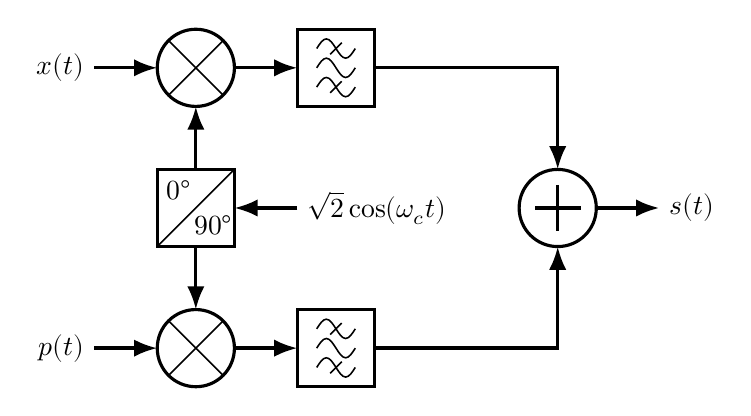
\begin{tikzpicture}[
					line width=0.2mm,
					node distance=8mm,
					arrow/.style={very thick, -Latex},
				]
					\node (div) [twoportsplitshape, circuitikz/t1={\SI{0}{\degree}}, circuitikz/t2={\SI{90}{\degree}}] {};
					\node (osc) [right=of div] {$\sqrt{2}\cos(\omega_ct)$};
					\node (add) [adder, right=of osc] {};
					\node (mixx) [mixer, above=of div] {};
					\node (mixp) [mixer, below=of div] {};
					\node (bndx) [bandpassshape, right=of mixx] {};
					\node (bndp) [bandpassshape, right=of mixp] {};
					
					\node (inx) [left=of mixx] {$x(t)$};
					\node (inp) [left=of mixp] {$p(t)$};
					\node (out) [right=of add] {$s(t)$};
					
					\draw[arrow] (inx) -- (mixx.west);
					\draw[arrow] (inp) -- (mixp.west);
					\draw[arrow] (osc.west) -- (div.east);
					\draw[arrow] (div.north) -- (mixx.south);
					\draw[arrow] (div.south) -- (mixp.north);
					\draw[arrow] (mixx.east) -- (bndx.west);
					\draw[arrow] (mixp.east) -- (bndp.west);
					\draw[arrow] (bndx.east) -- (bndx.east-|add.north) -- (add.north);
					\draw[arrow] (bndp.east) -- (bndp.east-|add.south) -- (add.south);
					\draw[arrow] (add) -- (out);
				\end{tikzpicture}
			\caption{Power spectrum illustrating single-quadrature upconversion.}
		\end{figure}
		\begin{equation}
			s(t)
			=
			x(t)
			\cos(\omega_ct)
			-
			p(t)
			\sin(\omega_ct)
			=
			\Re\left[
				\alpha(t)
				e^{+i\omega_c t}
			\right]
			\quad
			\text{with}
			\quad
			\alpha(t)
			=
			x(t)
			+
			ip(t)
		\end{equation}
	\end{frame}
	
	\begin{frame}{Dual-quadrature upconversion in the frequency domain}
		\begin{figure}
			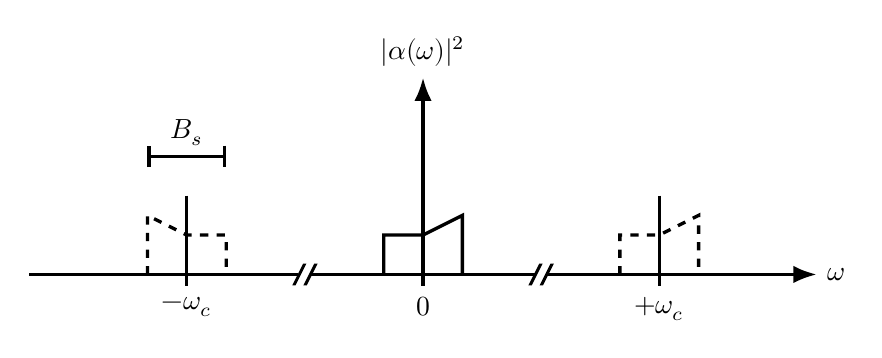
\begin{tikzpicture}
				\draw[very thick, -Latex] (0,0) -- ++(0,2.5) node[above] {$\abs{\alpha(\omega)}^2$};
				\draw[very thick, {-Bar[slant=.5]}] (-5,0) -- (-1.55,0);
				\draw[very thick, {Bar[slant=.5]-Bar[slant=.5]}] (-1.45,0) -- (1.45,0);
				\draw[very thick, {Bar[slant=.5]-Latex}] (1.55,0) -- (5,0) node[right] {$\omega$};
				\draw[very thick] (0,0) -- ++(0,-0.15) node[below] {$0$};
				
				\draw[very thick] (-0.5,0) -- ++(0,0.5) -- ++(0.5,0) -- ++(0.5,0.25) -- ++(0,-0.75);
				\draw[very thick] (3,1) -- ++(0,-1.15) node[below] {$+\omega_c$};
				\draw[very thick] (-3,1) -- ++(0,-1.15) node[below] {$-\omega_c$};
				\draw[very thick, dashed] (-3.5,0) -- ++(0,0.75) -- ++(0.5,-0.25) -- ++(0.5,0) -- ++(0,-0.5);
				\draw[very thick, dashed] (2.5,0) -- ++(0,0.5) -- ++(0.5,0) -- ++(0.5,0.25) -- ++(0,-0.75);
				
				\draw[Bar-Bar, very thick] (-3.5,1.5) -- ++(1,0) node[midway, above] {$B_s$};
			\end{tikzpicture}
			\caption{Power spectrum illustrating dual-quadrature upconversion.}
		\end{figure}
		\begin{equation}
			s(t)
			=
			\Re
			\int_{\omega_0-B_s/2}^{\omega_0+B_s/2}
			\frac{\dd{\omega}}{2\pi}
			\alpha(\omega-\omega_c)
			e^{+i\omega t}
		\end{equation}
	\end{frame}
	
	\begin{frame}{In-phase and quadrature modulator as dual-quadrature upconverter}
		\begin{figure}
			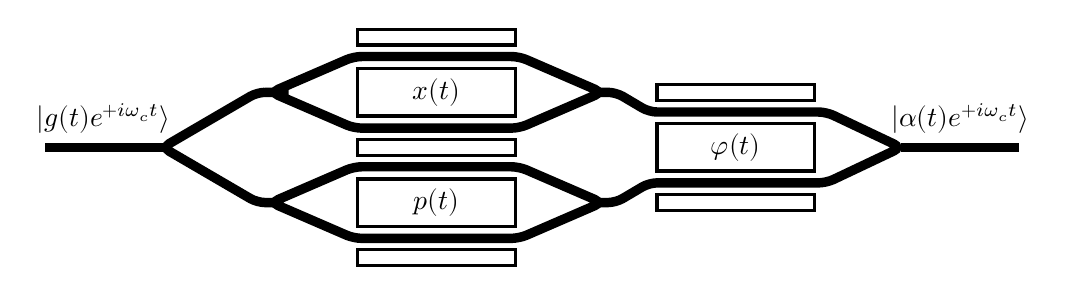
\begin{tikzpicture}[
				electrode/.style={very thick},
				waveguide/.style={line width=1.2mm, rounded corners=1mm},
			]
				\draw[electrode] (0,2.8) rectangle ++(2,0.2);
				\draw[electrode] (0,1.9) rectangle ++(2,0.6) node[pos=0.5] {$x(t)$};
				\draw[electrode] (0,1.4) rectangle ++(2,0.2);
				\draw[electrode] (0,0.5) rectangle ++(2,0.6) node[pos=0.5] {$p(t)$};
				\draw[electrode] (0,0) rectangle ++(2,0.2);
		
				\draw[waveguide] (1,0.8) node[draw, regular polygon, regular polygon sides=6, minimum width=1.05cm, xscale=4] (mzm1) {};
				\draw[waveguide] (1,2.2) node[draw, regular polygon, regular polygon sides=6, minimum width=1.05cm, xscale=4] (mzm2) {};
				
				\draw[electrode] (3.8,1.2) rectangle ++(2,0.6) node[pos=0.5] {$\varphi(t)$};
				\draw[electrode] (3.8,0.7) rectangle ++(2,0.2);
				\draw[electrode] (3.8,2.1) rectangle ++(2,0.2);
		
				\path (6.9,1.5) coordinate (out);
				\path (mzm1.east)
					++(-0.3,0) coordinate (a1) 
					++(0.2,0) coordinate (b1)
					(3.7,1.05) coordinate (c1) 
					++(2.25,0) coordinate (d1);
				\path (mzm2.east-|a1) coordinate (a2)
						(a2-|b1) coordinate (b2)
						(3.7,1.95) coordinate (c2)
						(c2-|d1) coordinate (d2);
		
				\draw[waveguide] (a1) -- (b1) -- (c1) -- (d1) -- (out) -- (d2) -- (c2) -- (b2) -- (a2);
		
				\draw[waveguide] (mzm1.west) ++(0.3,0) -- ++(-0.2,0) -- ++(-1.2,0.7) coordinate (in) -- ++(1.2,0.7) -- ++(0.2,0) -- ++(0.2,0) (mzm2.west);
				
				\draw[waveguide] (in) -- ++(-1.5,0) node[midway, above] {$\ket{g(t)e^{+i\omega_c t}}$};
				\draw[waveguide] (out) -- ++(1.5,0) node[midway, above] {$\ket{\alpha(t) e^{+i\omega_c t}}$};
			\end{tikzpicture}
			\caption{Drawing of an integrated in-phase and quadrature modulator.}
		\end{figure}
		\begin{equation}
			\ket{g(t)e^{+i\omega_c t}}
			\to
			\ket{\alpha(t)e^{+i\omega_c t}}
			\qquad
			\alpha(t)
			=
			g(t)
			\left[
				x(t)
				+
				iq(t)
			\right]
		\end{equation}
	\end{frame}
	
	\section{Coherent state receiver}
	
	\begin{frame}{Signal processing pipeline for symbol decoding}
		\begin{figure}
			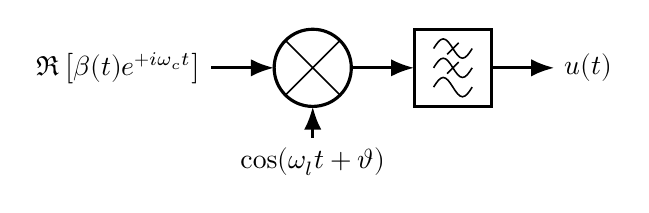
\begin{tikzpicture}[
				node distance=8mm,
				line width=0.2mm,
				arrow/.style={very thick, -Latex},
			]
				\node (in) {$\Re\left[\beta(t)e^{+i\omega_ct}\right]$};
				\node (mix) [mixer, right=of in] {};
				\node (low) [lowpassshape, right=of mix] {};
				\node (osc) [below=4mm of mix] {$\cos(\omega_lt+\vartheta)$};
				\node (out) [right=of low] {$u(t)$};
				
				\draw[arrow] (in) -- (mix.west);
				\draw[arrow] (mix.east) -- (low.west);
				\draw[arrow] (osc) -- (mix.south);
				\draw[arrow] (low.east) -- (out);
			\end{tikzpicture}
			\caption{Block diagram of single-quadrature downconversion.}
		\end{figure}
		\begin{figure}
			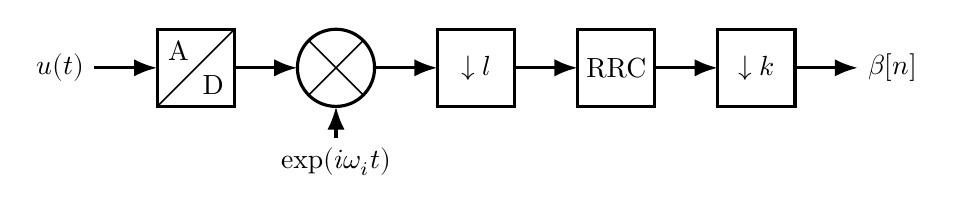
\begin{tikzpicture}[
				node distance=8mm,
				line width=0.2mm,
				arrow/.style={very thick, -Latex},
			]
				\node (in) {$u(t)$};
				\node (adc) [adcshape, right=of in] {};
				\node (mix) [mixer, right=of adc] {};
				\node (osc) [below=4mm of mix] {$\exp(i\omega_it)$};
				\node (down1) [twoportshape, t={$\downarrow l$}, right=of mix] {};
				\node (rrc) [twoportshape, t={RRC}, right=of down1] {};
				\node (down2) [twoportshape, t={$\downarrow k$}, right=of rrc] {};
				\node (out) [right=of down2] {$\beta[n]$};
				
				\draw[arrow] (in) -- (adc.west);
				\draw[arrow] (adc.east) -- (mix.west);
				\draw[arrow] (mix.east) -- (down1.west);
				\draw[arrow] (down1.east) -- (rrc.west);
				\draw[arrow] (rrc.east) -- (down2.west);
				\draw[arrow] (down2.east) -- (out.west);
				\draw[arrow] (osc.north) -- (mix.south);
			\end{tikzpicture}
			\caption{Block diagram of the analog-to-digital conversion and symbol-decoding.}
		\end{figure}
	\end{frame}

	\begin{frame}{Single-quadrature downconversion in the frequency domain}
		\begin{figure}
			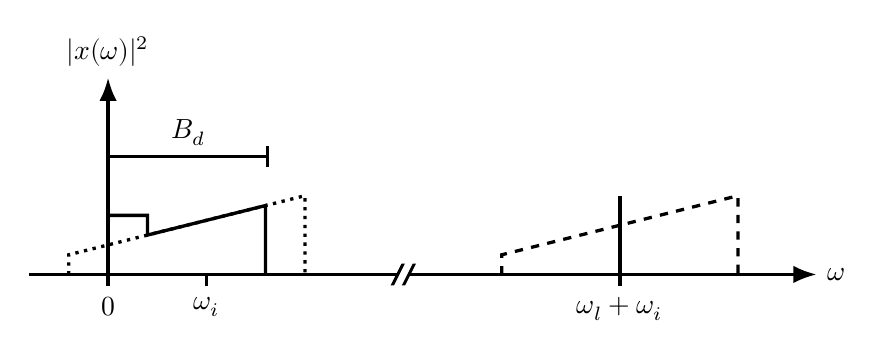
\begin{tikzpicture}
				\draw[very thick, -Latex] (0,0) -- ++(0,2.5) node[above] {$\abs{x(\omega)}^2$};
				\draw[very thick, {-Bar[slant=.5]}] (-1,0) -- (3.7,0);
				\draw[very thick, {Bar[slant=.5]-Latex}] (3.8,0) -- (9,0) node[right] {$\omega$};
		
				\draw[very thick] (0,0) -- ++(0,-0.15) node[below] {$0$};
				\draw[very thick] (1.25,0) -- ++(0,-0.15) node[below] {$\omega_i$};
				\draw[very thick] (6.5,0) -- ++(0,-0.15) node[below] {$\omega_l+\omega_i$};
				\draw[very thick] (6.5,0) -- ++(0,1);
		
				\draw[very thick, dashed] (5,0) -- ++(0,0.25) -- ++(3,0.75) -- ++(0,-1);
				\draw[very thick, dotted] (-0.5,0) -- ++(0,0.25) -- ++(3,0.75) -- ++(0,-1);
				\draw[very thick] (0,0.75) -- ++(0.5,0) -- ++(0,-0.25) -- ++(1.5,0.375) -- ++(0,-0.89);;
				
				\draw[-Bar, very thick] (0,1.5) -- ++(2.05,0) node[midway, above] {$B_d$};
			\end{tikzpicture}
			\caption{Power spectrum illustrating single-quadrature downconversion.}
		\end{figure}
		\begin{equation}
			u(t)
			=
			\Re
			\int_{0}^{+B_d/2}
			\frac{\dd{\omega}}{2\pi}
			\left[
				\beta(\omega+\omega_l)
				e^{+i\omega t}
				+
				\beta(\omega-\omega_l)^*
				e^{-i\omega t}
			\right]
			e^{-i\vartheta}
		\end{equation}
	\end{frame}
	
	\begin{frame}{Single-quadrature homodyne detection}
		\begin{figure}
			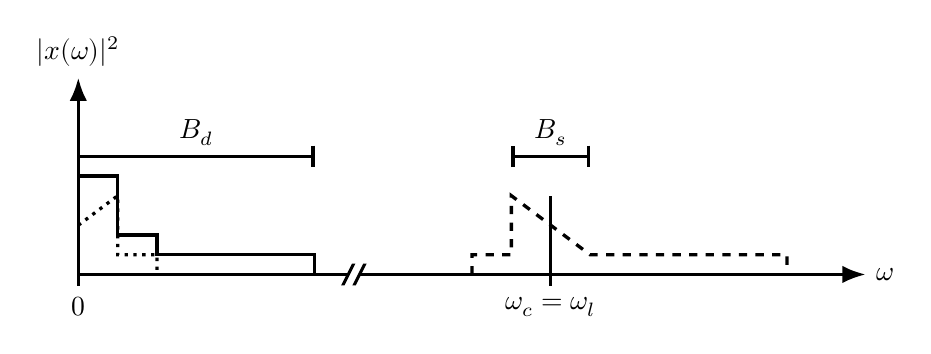
\begin{tikzpicture}
				\draw[very thick, -Latex] (0,0) -- ++(0,2.5) node[above] {$\abs{x(\omega)}^2$};
				\draw[very thick, {-Bar[slant=.5]}] (0,0) -- (3.45,0);
				\draw[very thick, {Bar[slant=.5]-Latex}] (3.55,0) -- (10,0) node[right] {$\omega$};
		
				\draw[very thick] (0,0) -- ++(0,-0.15) node[below] {$0$};
				\draw[very thick] (6,0) -- ++(0,-0.15) node[below] {$\omega_c=\omega_l$};
		
				\draw[very thick, dashed] (5,0) -- ++(0,0.25) -- ++(0.5,0) -- ++(0,0.75) -- ++(1,-0.75) -- ++(2.5,0) -- ++(0,-0.25);
				\draw[very thick] (6,0) -- ++(0,1);
		
				\draw[very thick] (0,1.25) -- ++(0.5,0) -- (0.5,0.5) -- ++(0.5,0) -- ++(0,-0.25) -- ++(2,0) -- ++(0,-0.25);
				\draw[very thick, dotted] (0,0.625) -- ++(0.5,0.375) -- (0.5,0.25) -- ++(0.5,0) -- ++(0,-0.25);
				
				\draw[Bar-Bar, very thick] (5.5,1.5) -- ++(1,0) node[midway, above] {$B_s$};
				\draw[-Bar, very thick] (0,1.5) -- ++(3,0) node[midway, above] {$B_d$};
			\end{tikzpicture}
			\caption{Power spectrum illustrating homodyne detection.}
		\end{figure}
		\begin{equation}
			u(t)
			=
			\Re
			\int_{0}^{+B_d/2}
			\frac{\dd{\omega}}{2\pi}
			\left[
				\beta(\omega)
				e^{+i\omega t}
				+
				\beta(\omega)^*
				e^{-i\omega t}
			\right]
			e^{-i\vartheta}
		\end{equation}
	\end{frame}
	
	\begin{frame}{Single-quadrature heterodyne detection}
		\begin{figure}
			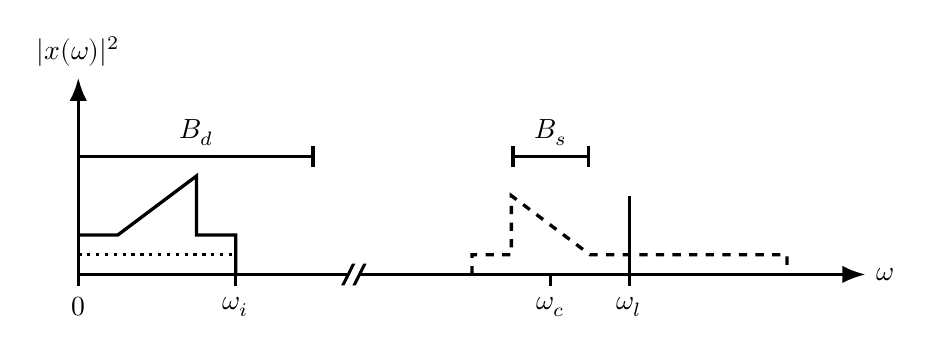
\begin{tikzpicture}
				\draw[very thick, -Latex] (0,0) -- ++(0,2.5) node[above] {$\abs{x(\omega)}^2$};
				\draw[very thick, {-Bar[slant=.5]}] (0,0) -- (3.45,0);
				\draw[very thick, {Bar[slant=.5]-Latex}] (3.55,0) -- (10,0) node[right] {$\omega$};
		
				\draw[very thick] (0,0) -- ++(0,-0.15) node[below] {$0$};
				\draw[very thick] (2,0) -- ++(0,-0.15) node[below] {$\omega_i$};
				\draw[very thick] (6,0) -- ++(0,-0.15) node[below] {$\omega_c$};
		
				\draw[very thick] (7,0) -- ++(0,-0.15) node[below] {$\omega_l$};
		
				\draw[very thick, dashed] (5,0) -- ++(0,0.25) -- ++(0.5,0) -- ++(0,0.75) -- ++(1,-0.75) -- ++(2.5,0) -- ++(0,-0.25);
				\draw[very thick] (7,0) -- ++(0,1);
				\draw[very thick] (0,0.5) -- ++(0.5,0) -- ++(1,0.75) -- ++(0,-0.75) -- ++(0.5,0) -- ++(0,-0.5);
				\draw[very thick, dotted] (0,0.25) -- ++(2,0) -- ++(0,-0.25);
				
				\draw[Bar-Bar, very thick] (5.5,1.5) -- ++(1,0) node[midway, above] {$B_s$};
				\draw[-Bar, very thick] (0,1.5) -- ++(3,0) node[midway, above] {$B_d$};
			\end{tikzpicture}
			\caption{Power spectrum illustrating heterodyne detection.}
		\end{figure}
		\begin{equation}
			u(t)
			=
			\Re
			\int_{0}^{+B_d/2}
			\frac{\dd{\omega}}{2\pi}
			\left[
				\beta(\omega+\omega_i)
				e^{+i\omega t}
				+
				\beta(\omega-\omega_i)^*
				e^{-i\omega t}
			\right]
			e^{-i\vartheta}
		\end{equation}
	\end{frame}
	
	\begin{frame}{Comparison homo- and heterodyne detection}
		\begin{table}
			\caption{Comparison of coherent receiver designs and their implications}
			\begin{tabular}{lccccc}
			    \toprule
			    & Homodyne (single) & Homodyne (dual) & Heterodyne \\
			    \midrule
			    Balanced detectors & \num{1} & \num{2} & \num{1} \\
			    Quadratures & \num{1} & \num{2} & \num{2} \\
			    Intermediate frequency & \multicolumn{2}{c}{$\omega_i=0$} & $\omega_i\neq 0$ \\
			    Optical complexity & Low & High & Low \\
			    Signal bandwidth & High & High & Low \\
			    LO synchronization & Frequency and phase & Frequency & Bandwidth \\
			    SNR & High & Low & Low \\
			    \bottomrule
			\end{tabular}
		\end{table}
	\end{frame}
	
	\begin{frame}{Balanced detector as single-quadrature downconverter}
		\begin{columns}[c, onlytextwidth]
			\column{0.45\textwidth}
			\vspace{-8mm}
			\begin{figure}
				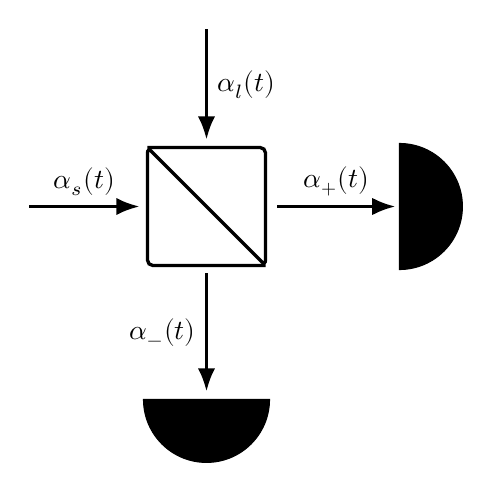
\begin{tikzpicture}[
					arrow/.style={very thick, -Latex},
				]
			        \draw[very thick, rounded corners=2pt] (0, 0) -- ++(1.5, 0) -- ++(0, -1.5) -- (0, 0) -- ++(0, -1.5) -- ++(1.5, 0);
			        
			        \draw[fill, rotate=-90, yshift=17mm, xshift=0.5mm] (1.5, 1.5) -- (1.5, 1.5) arc(0:180:0.8) --cycle;
			        \draw[fill=black, rotate=-180, yshift=17mm, xshift=-14.5mm] (1.5, 1.5) -- (1.5, 1.5) arc(0:180:0.8) --cycle;

			        \draw[arrow] (-1.5, -0.75) -- ++(1.4, 0) node[midway, above] {$\alpha_s(t)$};
			        \draw[arrow] (0.75, 1.5) -- ++(0, -1.4) node[midway, right] {$\alpha_l(t)$};
			        \draw[arrow] (0.75, -1.6) -- ++(0,-1.5) node[midway, left] {$\alpha_-(t)$};
			        \draw[arrow] (1.65, -0.75) -- ++(1.5, 0) node[midway, above] {$\alpha_+(t)$};
			    \end{tikzpicture}
			    \caption{Electro-optical setup for balanced detection.}
			\end{figure}

			\column{0.55\textwidth}
			\begin{block}{Differential photocurrent signal}
				\begin{equation}
					i(t)
					\propto
					\Re
					\int_{-B_d/2}^{+B_d/2}
					\frac{\dd{\omega}}{2\pi}
					\beta(\omega+\omega_l)
					e^{+i(\omega t+\vartheta)}
				\end{equation}
	        \end{block}

			\begin{block}{Phase-rotated quadrature operator}
				\begin{equation}
					\hat{X}(t)
					=
					\int_{-\infty}^{+\infty}
					\frac{\dd{\omega}}{2\pi}
					\left[
						\hat{a}(\omega)
						e^{-i(\omega t+\vartheta)}
						+
						\text{H.c.}
					\right]
				\end{equation}
			\end{block}

			\begin{block}{Frequency-converted annihilation operator}
				\begin{equation}
					\hat{U}^\dagger
					\hat{a}(\omega)
					\hat{U}
					=
					\sum_{m\in\mathbb{Z}}
					J_m(\theta)
					\hat{a}(\omega+m\omega_l)
					e^{-im\vartheta}
				\end{equation}
			\end{block}
		\end{columns}
	\end{frame}
	
	\section{Conclusion and outlook}
	
	\begin{frame}{Summary}
		\begin{itemize}
			\item Introduction to CV-QKD as a mechanism for secure key distribution.
			\item Raised awareness to dependence of transmissions.
			\item Introduction to a software-defined coherent transmission system.
			\item Introduction to concepts and methods from communication engineering.
			\item Extension of coherent transmission system to quantum regime.
		\end{itemize}
	\end{frame}
	
	\begin{frame}{Additional topics covered in the thesis}
		\begin{itemize}
			\item Overview and comparison of DV- and CV-QKD protocols including post processing.
			\item Derivation of continuous-mode quantum theory of light rooted in quantum field theory.
			\item Summary of quantum models for the most important (electro-)optical components as building blocks for communication system.
		\end{itemize}		
	\end{frame}
	
	\begin{frame}{Outlook}
		\begin{itemize}
			\item Noise model for measurements.
			\item Comparison of image band and squeezing attack.
			\item Further transfer of telecommunication methods, e.g., orthogonal frequency-division multiplexing (OFDM).
			\item Properties of frequency-squeezed states.
			\item Equivalence of tensor-product with continuous-time coherent state transmission.
		\end{itemize}
	\end{frame}

\end{document}